%========================================================
% Reusable academic paper template
% Preserves the overall look and feel of the uploaded draft
% while removing the original paper-specific content.
%
% Quick start:
% 1. Replace the metadata block below.
% 2. Set \blindtrue for anonymized (blind-review) output, or \blindfalse to show authors.
% 3. Replace the sample text, tables, and figures.
% 4. Replace the .bib file with your own references.
% 5. Compile with: pdflatex -> bibtex -> pdflatex -> pdflatex
%========================================================

\documentclass[hidelinks,12pt]{article}

\usepackage{graphicx}
\usepackage{setspace}
\usepackage[svgnames]{xcolor}
\usepackage[colorlinks=true,citecolor=DarkBlue,linkcolor=Maroon]{hyperref}
\usepackage{fancyhdr}
\usepackage{natbib}
\usepackage[format=hang,font=large,labelfont=bf]{caption}
\usepackage{tabularx}
\usepackage{booktabs,multicol,multirow}
\usepackage[margin=2cm]{geometry}
\usepackage{array}
\usepackage{amsmath}
\usepackage{enumitem}
\usepackage[toc,page]{appendix}

\captionsetup[table]{labelsep=period}
\captionsetup[figure]{labelsep=period}

\newcolumntype{Y}{>{\raggedleft\arraybackslash}X}
\newcolumntype{L}[1]{>{\raggedright\let\newline\\\arraybackslash\hspace{0pt}}m{#1}}

\def\sym#1{\ifmmode^{#1}\else\(^{#1}\)\fi}

% Capitalized autoref names for clickable cross-references
\renewcommand{\figureautorefname}{Figure}
\renewcommand{\tableautorefname}{Table}
\renewcommand{\sectionautorefname}{Section}
\renewcommand{\subsectionautorefname}{Section}
\newcommand{\propositionautorefname}{Proposition}
\newcommand{\hypothesisautorefname}{Hypothesis}
\newcommand{\appendixautorefname}{Appendix}

\newcommand{\runningtitle}{Academic Paper Template}
\newcommand{\papertitle}{Reusable Academic Paper Template: Example Layout for Empirical Research}
\newcommand{\paperauthorone}{First Author}
\newcommand{\paperauthortwo}{Second Author}
\newcommand{\paperaffilone}{Department of Finance, University A}
\newcommand{\paperaffiltwo}{Department of Economics, University B}
\newcommand{\paperemailone}{first.author@university.edu}
\newcommand{\paperemailtwo}{second.author@university.edu}

\newif\ifblind
\blindfalse % change to \blindtrue for anonymized (blind-review) output

\newcommand{\floatnotes}[1]{%
\begin{quotation}
\noindent \scriptsize #1
\end{quotation}
}

\renewcommand{\baselinestretch}{1.9}
\setlength{\textheight}{8.6in}
\setlength{\textwidth}{6.3in}
\setlength{\oddsidemargin}{0.1in}
\setlength{\topmargin}{-0.30in}
\setlength{\footnotesep}{10.0pt}
\setlength{\headheight}{14.5pt}

\pagestyle{fancyplain}
\fancyhf{}
\lhead{\textbf{\runningtitle}}
\rhead{\thepage}
\renewcommand{\headrulewidth}{0.4pt}
\renewcommand{\footrulewidth}{0pt}

\title{\bf \papertitle\\
\vspace*{-20pt}}
\author{}
\date{}

\begin{document}

\maketitle
\thispagestyle{empty}

\ifblind\else
\vspace{-1.5em}
\begin{center}
\paperauthorone\\
\textit{\paperaffilone}\\
\href{mailto:\paperemailone}{\paperemailone}
\vspace{0.7em}

\paperauthortwo\\
\textit{\paperaffiltwo}\\
\href{mailto:\paperemailtwo}{\paperemailtwo}
\end{center}
\vspace{1.0em}
\fi

\begin{abstract}
\vspace{0pt}
\setstretch{1.15}
This document is a reusable template that keeps the general appearance of the uploaded draft while removing the original paper-specific material. It includes a sample title page, abstract, section structure, equations, hypotheses, references, tables, figures, and an appendix. The example prose is written around a stylized empirical finance question on disclosure quality and financing costs, but every number, coefficient, table entry, and graphic is illustrative only. Replace the metadata, narrative, variable names, sample description, notes, and bibliography with your own project-specific content before submission.
\end{abstract}

\setstretch{1.9}

\vspace{32pt}
{\noindent JEL Classification: } G10, G30, C23\\
Keywords: academic template; empirical finance; disclosure; financing costs

\newpage
\setcounter{page}{1}

%--------------------------------------------------------
\section{Introduction}
\label{sec:intro}

A strong introduction usually does four things in quick succession: it states the research question, explains why the question matters, positions the paper relative to the literature, and previews the empirical design and the main findings. This template illustrates that structure with placeholder content built around a stylized relation between disclosure quality and financing costs. Replace the topic, motivation, and contribution statements with the central question in your own paper.

For illustration, suppose the paper studies whether better disclosure lowers financing frictions by improving investor understanding and reducing information asymmetry. That framing fits naturally with prior work on disclosure and the cost of capital, including \citet{botosan1997disclosure}, \citet{healy2001information}, and \citet{lambert2007accounting}. A finance paper might then connect the question to broader asset-pricing or corporate-finance themes such as risk premia, monitoring, or capital structure, perhaps citing benchmark references like \citet{fama1993common} or \citet{jensen1976theory}.

A second paragraph in the introduction typically explains the research design at a high level. Here, the placeholder design uses panel regressions with firm and year fixed effects, standard controls, and clustered standard errors following \citet{petersen2009estimating}. It also flags endogeneity concerns and previews the kinds of robustness checks discussed by \citet{angrist2009mostly}.\footnote{Use footnotes sparingly. They work best for brief institutional details, measurement clarifications, or secondary discussion that would otherwise interrupt the main argument.}

A third paragraph often summarizes the paper's contributions. In a completed draft, this is where you would explain what is new relative to prior work, why the data or identification strategy is informative, and how the magnitudes matter economically. The sample tables/figures at the end of the document show common formatting choices for descriptive statistics, baseline regressions, heterogeneity tests, and visual summaries. For example, \autoref{tab:summary} presents summary statistics, \autoref{tab:baseline} presents a baseline regression layout, and \autoref{fig:binned_scatter} shows a standard binned-scatter figure.

The remainder of the paper proceeds as follows. \autoref{sec:literature} illustrates how to position the study in the literature and develop hypotheses. \autoref{sec:data} describes the sample and variable construction. \autoref{sec:design} presents an example empirical specification. \autoref{sec:results} and \autoref{sec:additional} show a typical flow for main results, heterogeneity, and robustness. The appendix provides an example supplementary section and a variable-definition table.

%--------------------------------------------------------
\section{Related Literature and Hypothesis Development}
\label{sec:literature}

\subsection{Related Literature}

A literature review should usually identify two or three specific strands of work rather than reciting a long list of citations. In this example, the first strand concerns the role of disclosure and information quality in financing outcomes \citep{botosan1997disclosure,healy2001information,lambert2007accounting}. The second strand concerns empirical measurement and interpretation of financing frictions, capital costs, or expected returns \citep{fama1993common}. A third strand can cover the econometric choices most relevant for the design, including fixed effects, clustered standard errors, and endogeneity \citep{petersen2009estimating,angrist2009mostly}.

The goal is not simply to cite papers, but to explain how the current study differs from or extends them. You may be testing a new mechanism, using richer micro-level data, examining a different institutional setting, or quantifying heterogeneity that earlier papers could not observe. If your contribution is methodological, this is also the place to state how the design improves on prior identification or measurement choices.

\subsection{Hypothesis Development}

This subsection typically translates the conceptual mechanism into testable predictions. In the running example, higher disclosure quality may reduce uncertainty about future cash flows, improve monitoring, and expand access to external capital. Those channels imply a negative association between disclosure quality and financing costs.

\noindent \textbf{Hypothesis 1.} Higher disclosure quality is associated with lower financing costs.

A useful second hypothesis often addresses cross-sectional heterogeneity. For example, the effect of disclosure may be stronger when firms are financially constrained, have limited analyst coverage, or operate in settings where outside investors rely more heavily on public information.

\noindent \textbf{Hypothesis 2.} The negative association between disclosure quality and financing costs is stronger when external financing frictions are more severe.

If the paper has a formal model or a richer institutional setting, that material can appear here as an additional subsection. The template is intentionally flexible: you can keep this section brief, or expand it into a full theory or institutional-background section as needed.

%--------------------------------------------------------
\section{Data and Variable Construction}
\label{sec:data}

\subsection{Sample Construction}

A data section generally explains the sample period, the data sources, the merge procedure, and the filters applied to construct the final sample. The placeholder sample here contains 2,400 firm-year observations from 2010 through 2022. In your own draft, this paragraph should identify the primary database, describe how missing observations are handled, explain winsorization or trimming choices, and justify the final sample restrictions.

It is often useful to preview the sample with one table and one figure. \autoref{tab:summary} provides an example summary-statistics table with a second panel for correlations. \autoref{fig:histograms} provides an example descriptive figure with two panels. Both are purely illustrative; replace the numbers and notes with content that matches your actual data.

\subsection{Variable Definitions}

The main dependent variable in the example is \textit{Financing Cost}, measured in percentage points. The focal explanatory variable is \textit{Disclosure Quality}, scaled from 0 to 100. The remaining controls are standard placeholders for firm size, leverage, profitability, growth opportunities, asset tangibility, and analyst coverage. \autoref{tab:appendix_variables} shows one way to format a concise variable-definition table.

When writing your own variable section, define variables precisely enough that a reader could replicate them. If the variable is transformed, indicate whether you use logs, percentiles, indicator variables, standardized scores, or industry-adjusted measures. If the construction is lengthy, summarize it briefly here and move the mechanical detail to the appendix.

%--------------------------------------------------------
\section{Empirical Design}
\label{sec:design}

A standard panel specification can be written as follows:
\begin{equation}
\label{eq:baseline}
\begin{aligned}
\textit{FinancingCost}_{i,t}
&=
\alpha
+
\beta\,\textit{DisclosureQuality}_{i,t-1}
+
\Gamma'X_{i,t-1}
\\
&\quad
+
\mu_i
+
\lambda_t
+
\varepsilon_{i,t},
\end{aligned}
\end{equation}
where $X_{i,t-1}$ is a vector of controls, $\mu_i$ denotes firm fixed effects, and $\lambda_t$ denotes year fixed effects. In a completed paper, use the notation that matches your setting and define each term immediately after the equation.

To test cross-sectional predictions, you can extend Equation~\eqref{eq:baseline} with interaction terms:
\begin{equation}
\label{eq:interaction}
\begin{aligned}
\textit{FinancingCost}_{i,t}
&=
\alpha
+
\beta\,\textit{DisclosureQuality}_{i,t-1}
\\
&\quad
+
\delta\left(\textit{DisclosureQuality}_{i,t-1}\times \textit{HighConstraint}_{i,t-1}\right)
\\
&\quad
+
\Gamma'X_{i,t-1}
+
\mu_i
+
\lambda_t
+
\varepsilon_{i,t}.
\end{aligned}
\end{equation}

This is also a good place to explain your inference choices. For example, a finance paper may cluster standard errors by firm and year following \citet{petersen2009estimating}. If your design relies on an event study, a difference-in-differences design, or an instrumental variable, state that clearly here and give the identifying variation in plain language before moving to the results.

%--------------------------------------------------------
\section{Main Results}
\label{sec:results}

\autoref{tab:baseline} illustrates a common regression layout. In the example, the coefficient on disclosure quality is negative and statistically significant across specifications, consistent with Hypothesis~1. The first column shows a parsimonious relation. Subsequent columns add controls and fixed effects. In a real paper, this text would interpret the coefficient magnitudes, discuss identification, and connect the results back to the economics of the question.

\autoref{fig:binned_scatter} provides a nonparametric companion to the regression table. Binned-scatter plots are often useful because they show the broad shape of the relation without forcing the reader to infer it from coefficients alone. In your own draft, the figure note should state exactly what has been residualized, which sample restrictions are imposed, and whether the fitted line is linear, quadratic, or produced by another smoother.

One paragraph in the main-results section should usually address economic magnitude, not just statistical significance. For instance, if a ten-point increase in disclosure quality corresponds to a 12 to 18 basis-point reduction in financing costs, say so plainly and benchmark the effect against the sample mean or the interquartile range. If the magnitude is small, explain why it may still matter in the setting you study.

%--------------------------------------------------------
\section{Additional Analyses and Heterogeneity}
\label{sec:additional}

\autoref{tab:heterogeneity} shows an example heterogeneity table using interaction terms. The placeholder coefficients suggest that disclosure quality matters more for firms facing tighter financing conditions or weaker external information environments. \autoref{fig:heterogeneity} then visualizes that heterogeneity using fitted values from the interaction specification.

You can repurpose this section for mechanisms, subsample analysis, event-time dynamics, falsification tests, or institutional splits. The key is to keep the logic disciplined: each additional result should answer a specific question raised by the theory, identification, or external validity of the baseline finding.

%--------------------------------------------------------
\section{Robustness and Identification}
\label{sec:robustness}

A typical robustness section addresses alternative variable definitions, omitted-variable concerns, sample composition, and inference choices. Depending on the project, this may include lag structures, additional fixed effects, matched samples, entropy balancing, placebo tests, or alternative clustering schemes. If the design is observational, it is usually worth stating candidly what sources of endogeneity remain after the baseline controls and fixed effects.

This is also where you can explain any differences between your main specification and the versions reported in the appendix or Internet Appendix. If the paper has many robustness checks, use a clear organizing principle rather than presenting them as a long undifferentiated list.

%--------------------------------------------------------
\section{Conclusion}
\label{sec:conclusion}

The conclusion should restate the research question, summarize the main evidence, and explain the broader implication without merely repeating the abstract. In the present template, the broader purpose is practical: it provides a clean academic-paper shell that preserves the style of the uploaded draft while stripping out the original content. Replace the placeholder discussion with a concise summary of your actual contribution, limitations, and avenues for future work.

%--------------------------------------------------------
\appendix
\section{Additional Details and Variable Definitions}
\label{sec:appendix}

Appendix sections are useful for measurement detail, supplementary figures, robustness checks, and institutional background that is important but too lengthy for the main text. \autoref{tab:appendix_variables} shows one common appendix layout. \autoref{fig:appendix_hist} gives a simple example of an appendix figure.

A longer appendix might also report alternative variable definitions, additional sample screens, timing conventions, or robustness tables that would otherwise interrupt the flow of the main text. If your paper has a separate Internet Appendix, this section can briefly explain what is included there and how it relates to the main manuscript.

\bibliographystyle{jf}
\bibliography{template_references}

%--------------------------------------------------------
% Example figures and tables placed after the references,
% matching the overall structure of the source draft.
% Move them inline if your target journal prefers that layout.
%--------------------------------------------------------

\clearpage
\begin{figure}[!htbp]
\caption{Histograms of Financing Cost and Disclosure Quality}
\label{fig:histograms}\vspace{-2.5ex}
\floatnotes{This figure provides a sample two-panel descriptive layout. Panel A plots the distribution of the dependent variable, financing cost, and Panel B plots the distribution of the main explanatory variable, disclosure quality. Replace the image files and the note with your own sample-specific content.}
\centering
\textbf{Panel A. Financing Cost}\\
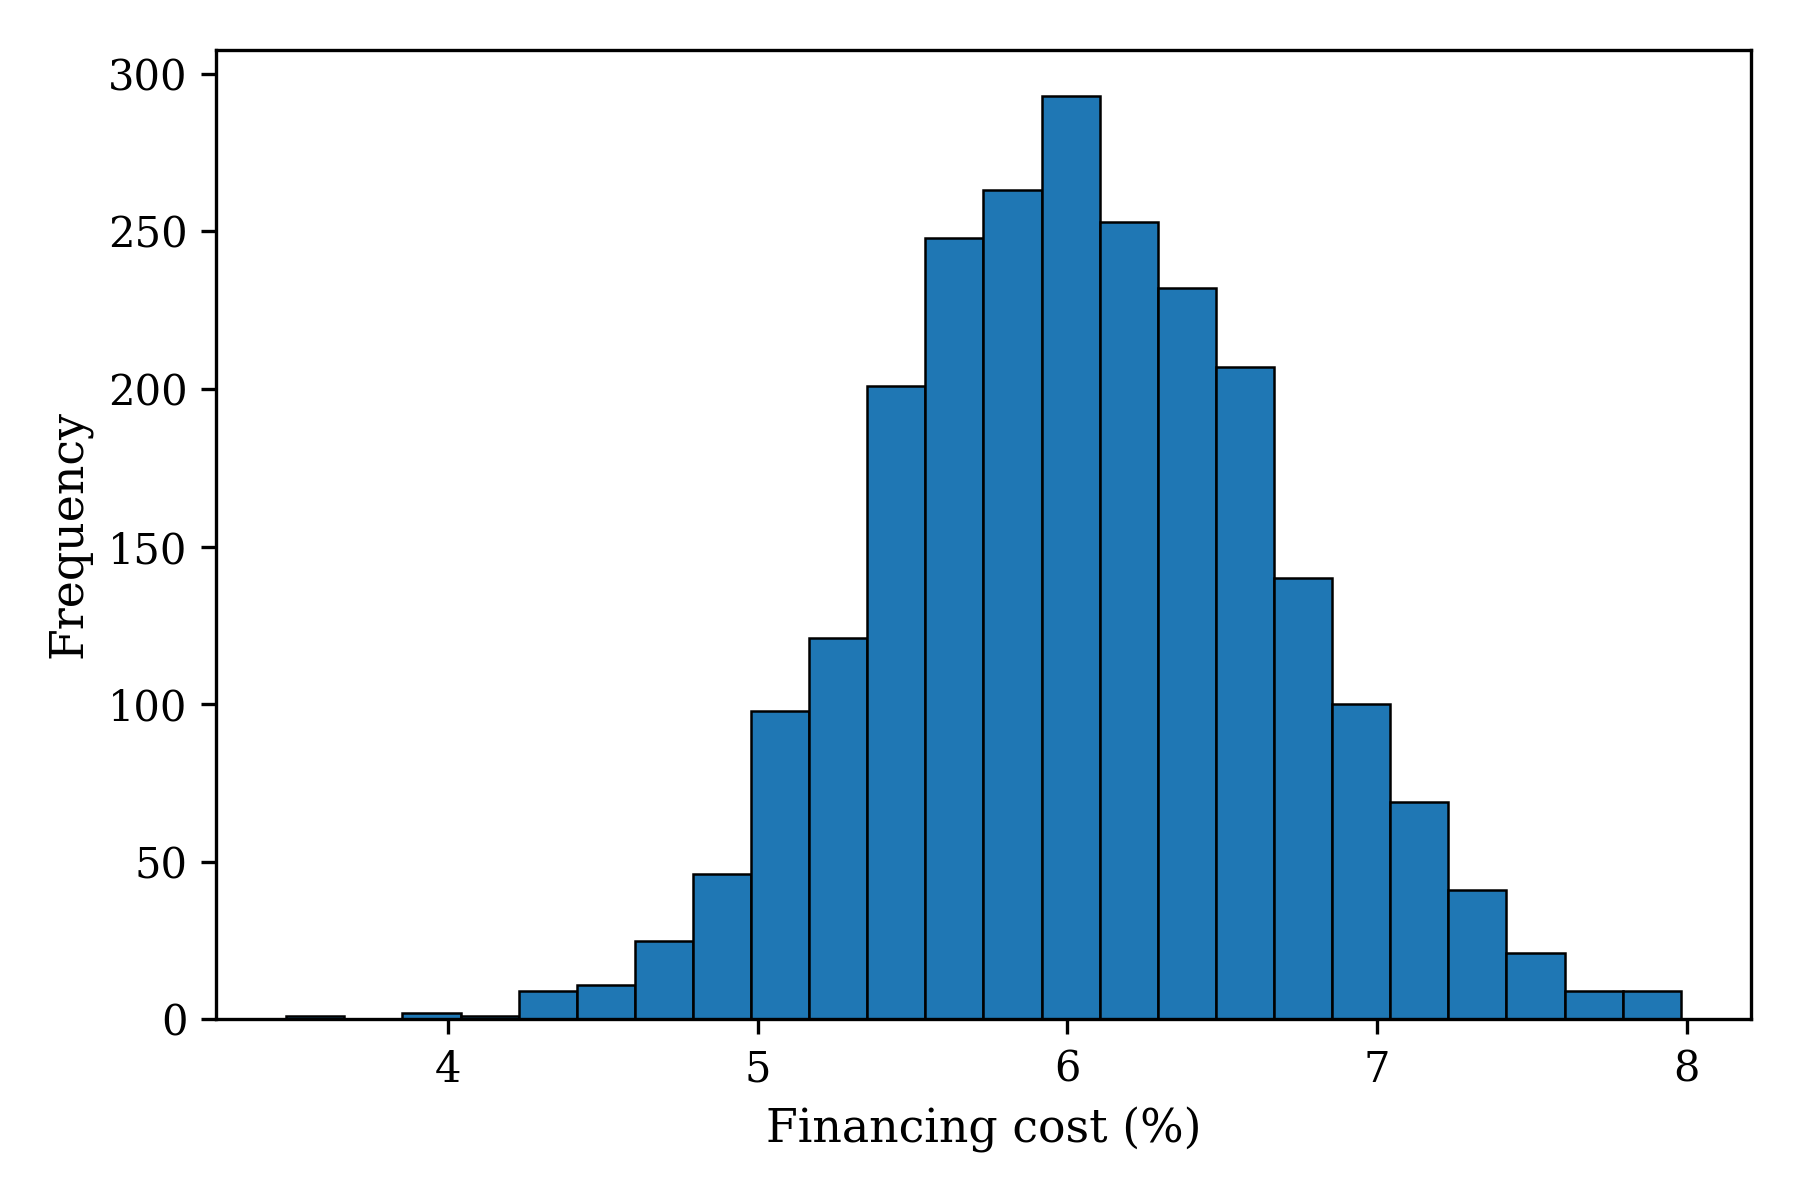
\includegraphics[width=10.16cm,height=6.77cm]{./images/fig1a.png}\\
\textbf{Panel B. Disclosure Quality}\\
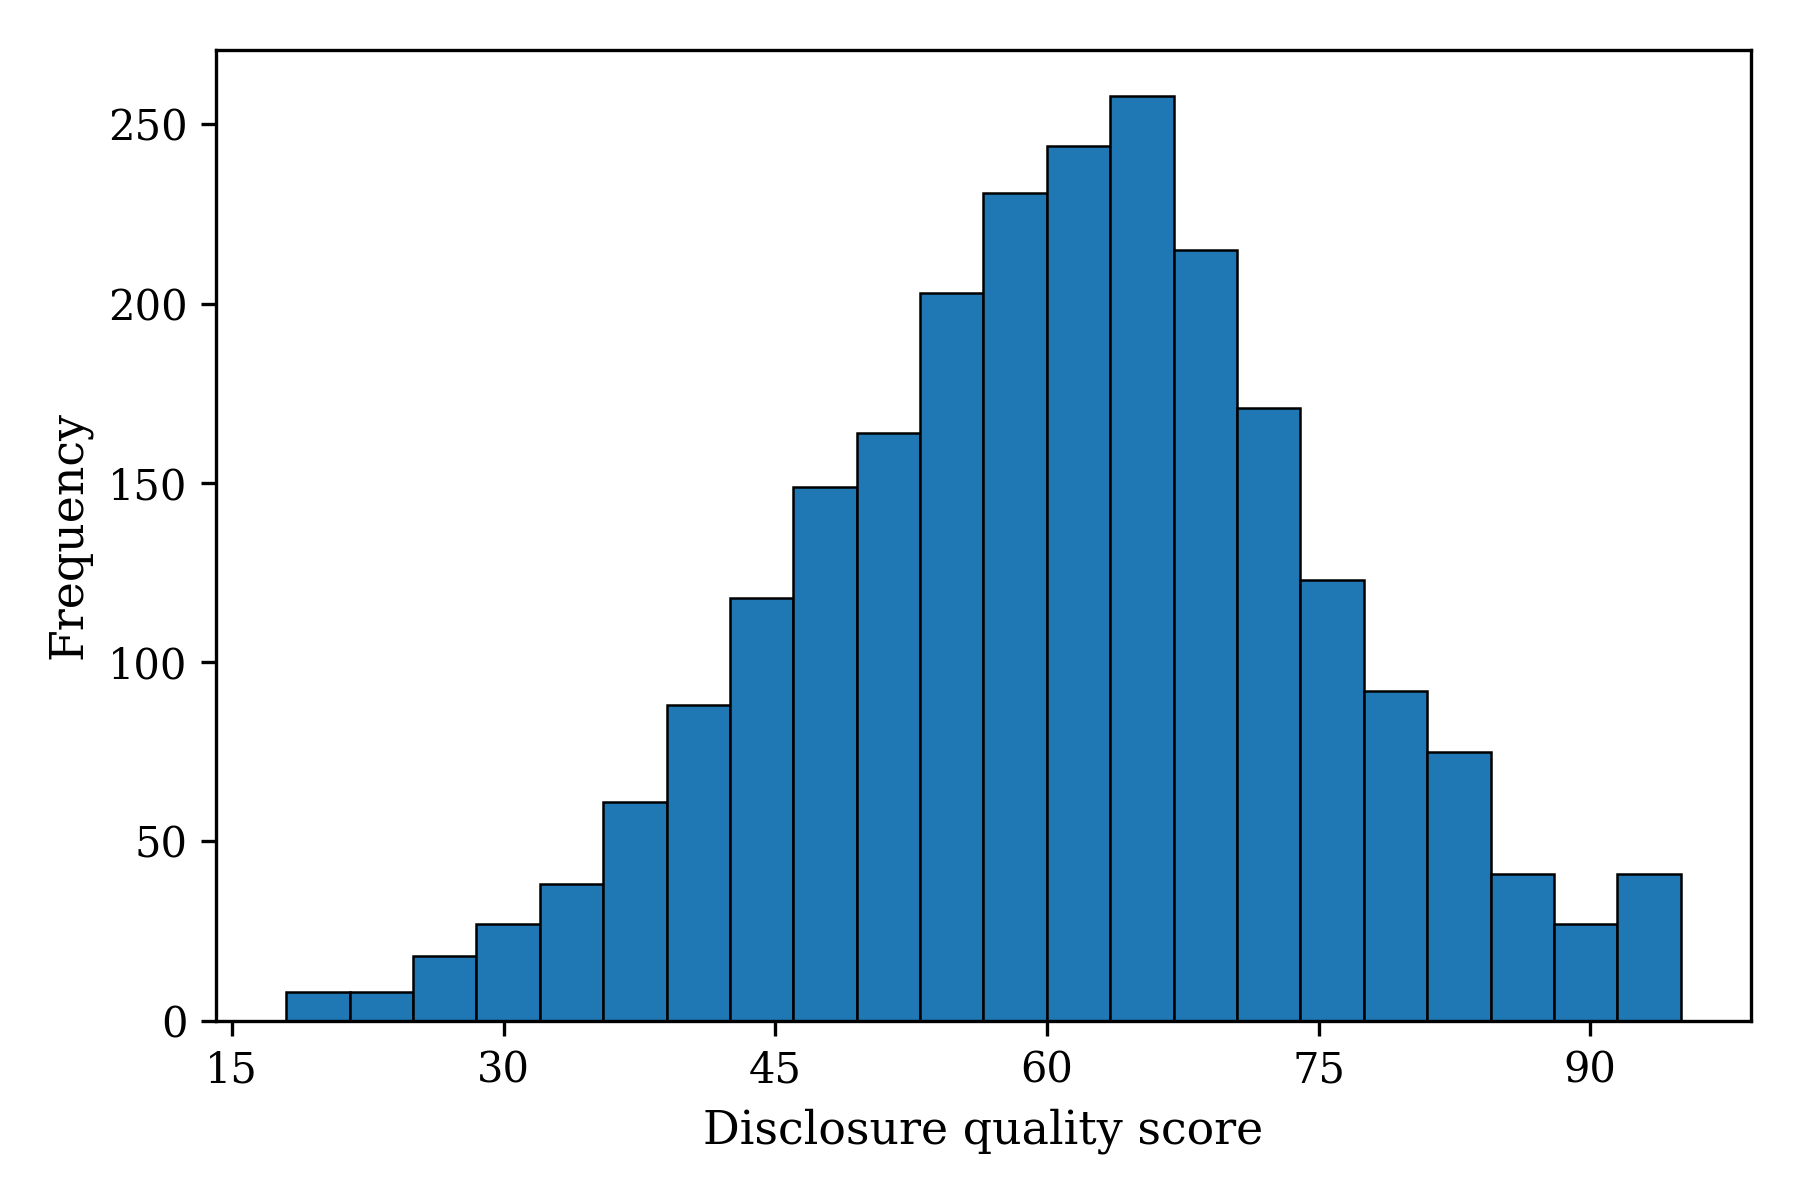
\includegraphics[width=10.16cm,height=6.77cm]{./images/fig1b.png}
\end{figure}

\clearpage
\begin{figure}[!htbp]
\caption{Binned Scatter Plot of Financing Cost and Disclosure Quality}
\label{fig:binned_scatter}\vspace{-2.5ex}
\floatnotes{This figure illustrates a common visual summary for the relation between the dependent variable and the main explanatory variable. The points show binned means and the solid line shows a fitted quadratic relation. In your own paper, specify whether fixed effects or controls have been partialled out before constructing the plot.}
\centering
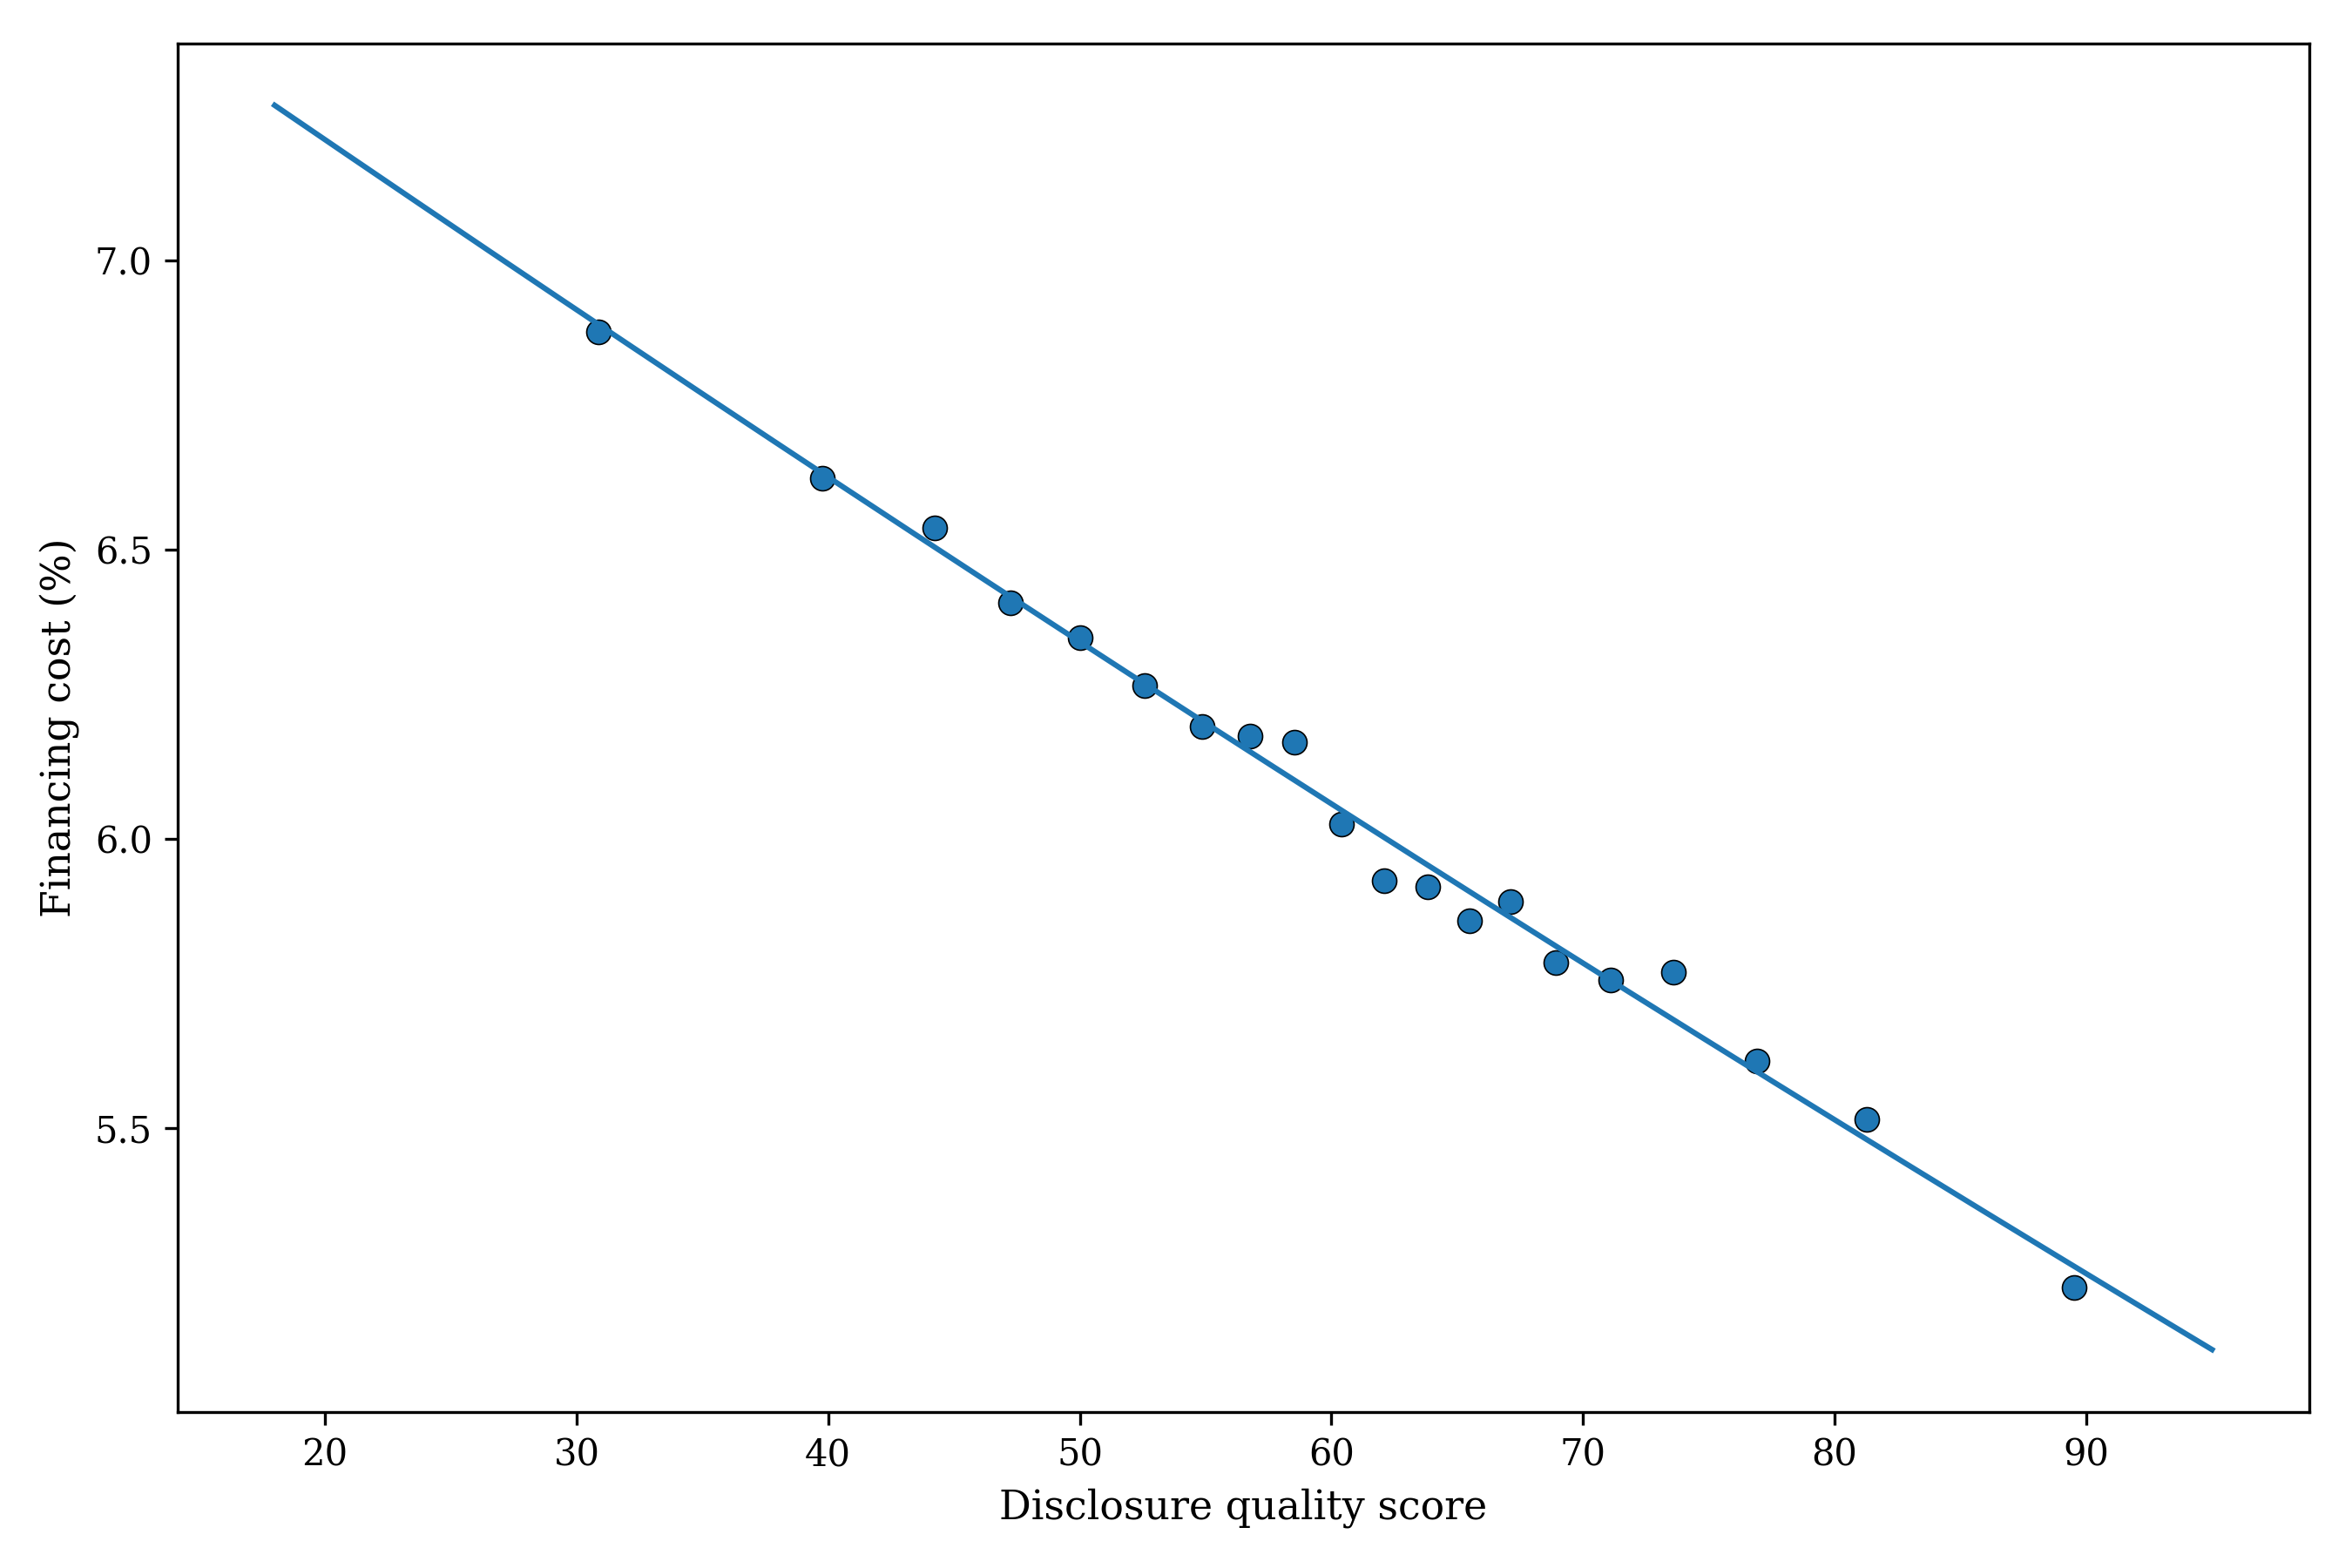
\includegraphics[width=15.24cm,height=10.16cm]{./images/fig2.png}
\end{figure}

\clearpage
\begin{figure}[!htbp]
\caption{Predicted Financing Cost by Disclosure Quality and Financial Constraint Status}
\label{fig:heterogeneity}\vspace{-2.5ex}
\floatnotes{This figure shows one way to present cross-sectional heterogeneity. The lines can be interpreted as fitted values from the interaction specification in \autoref{tab:heterogeneity}. Replace the group labels, fitted values, and confidence intervals so they match your own empirical setting.}
\centering
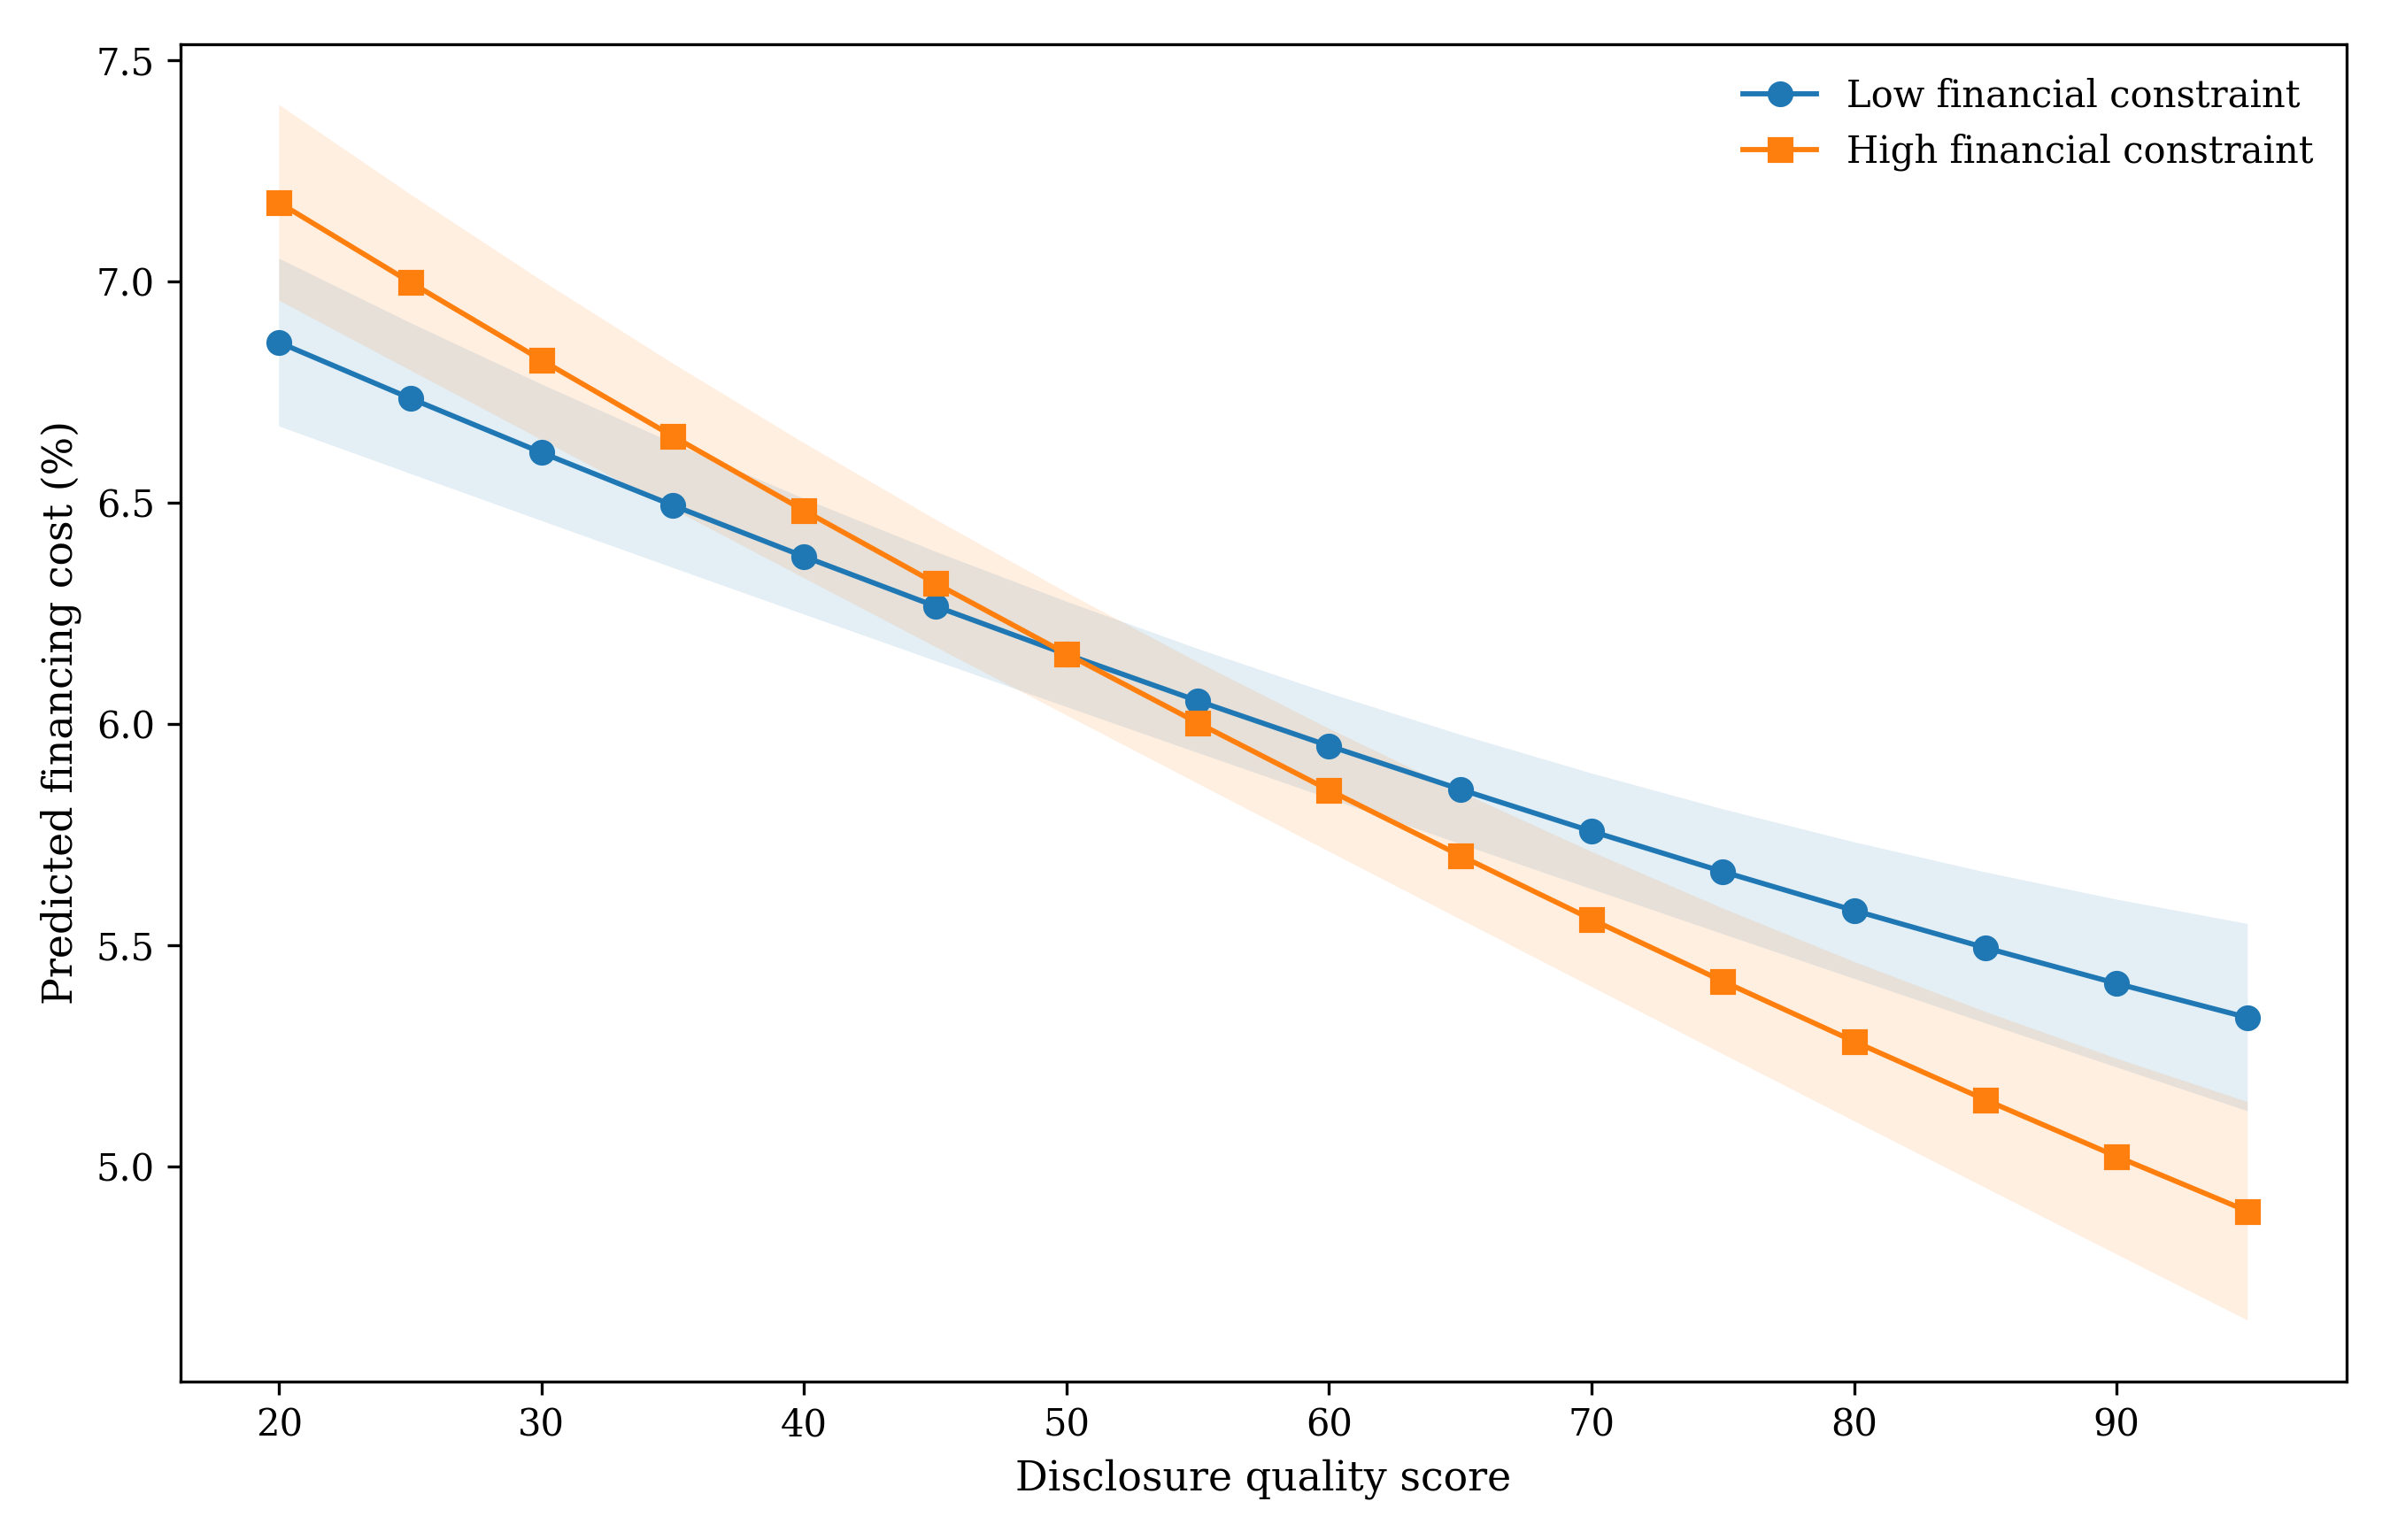
\includegraphics[width=15.24cm,height=9.6cm]{./images/fig3.png}
\end{figure}

\clearpage
\begin{figure}[!htbp]
\caption{Appendix Figure: Distribution of Regression Residuals}
\label{fig:appendix_hist}\vspace{-2.5ex}
\floatnotes{Appendix figures are useful for diagnostics, supplementary descriptive evidence, or alternative specifications. This residual histogram is included only as a formatting example.}
\centering
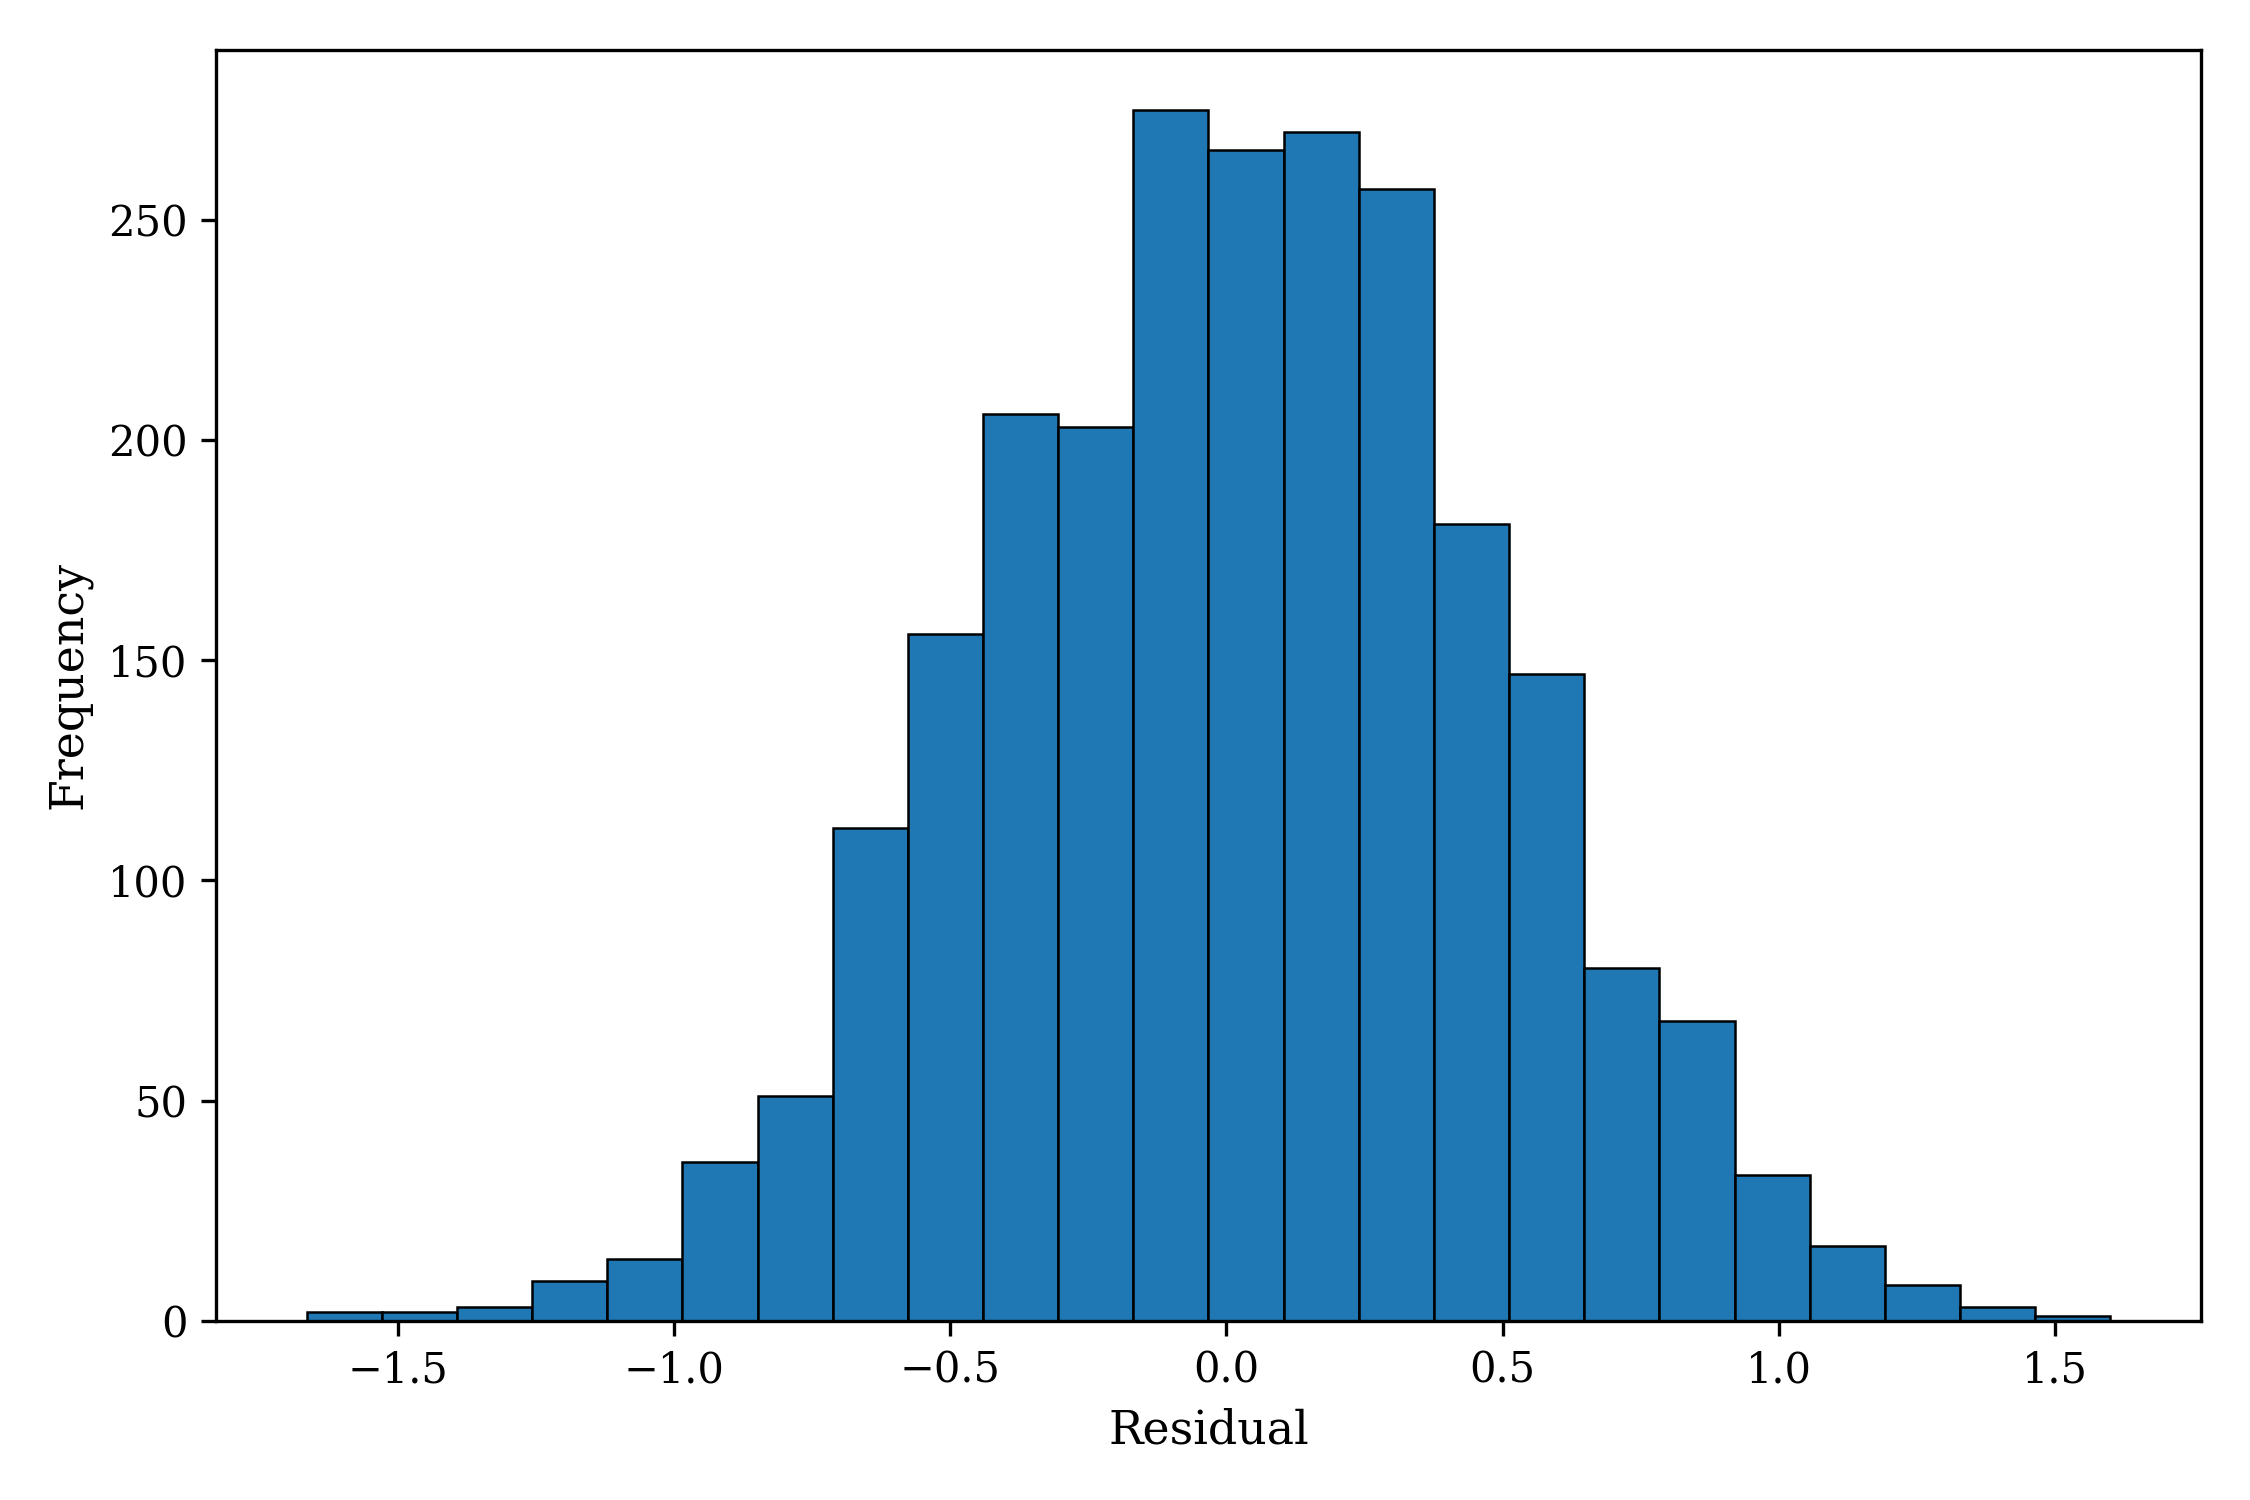
\includegraphics[width=12.8cm,height=8.5cm]{./images/figA1.png}
\end{figure}

\clearpage
\begin{table}[!htbp]
\centering
\caption{Summary Statistics}
\label{tab:summary}\vspace{-2.5ex}
\floatnotes{This table illustrates a standard summary-statistics layout with an optional second panel for correlations. Replace the variable labels, sample description, and descriptive moments with your own data. Panel A reports means, standard deviations, and selected distributional statistics. Panel B reports simple pairwise correlations among core variables.}
\setlength{\tabcolsep}{5pt}
\small

\textbf{Panel A. Descriptive Statistics}
\begin{tabularx}{\textwidth}{@{}Xrrrrrr@{}}
\\
\toprule
\textbf{Variable} & \textbf{Mean} & \textbf{SD} & \textbf{P25} & \textbf{Median} & \textbf{P75} & \textbf{N} \\
\midrule
Financing Cost (\%) & 5.87 & 1.12 & 5.08 & 5.83 & 6.61 & 2,400 \\
Disclosure Quality & 61.40 & 14.20 & 51.00 & 62.00 & 72.00 & 2,400 \\
Ln(Assets) & 7.93 & 1.12 & 7.14 & 7.88 & 8.70 & 2,400 \\
Leverage & 0.29 & 0.17 & 0.15 & 0.28 & 0.41 & 2,400 \\
Profitability & 0.11 & 0.07 & 0.06 & 0.10 & 0.15 & 2,400 \\
Market-to-Book & 1.84 & 0.76 & 1.29 & 1.73 & 2.24 & 2,400 \\
Tangibility & 0.31 & 0.16 & 0.18 & 0.30 & 0.42 & 2,400 \\
Analyst Coverage & 12.70 & 7.80 & 6.00 & 11.00 & 18.00 & 2,400 \\
\bottomrule
\\
\end{tabularx}

\medskip
\textbf{Panel B. Correlation Matrix}

\footnotesize
\begin{tabularx}{\textwidth}{@{}X*{6}{r}@{}}
\\
\toprule
 & (1) & (2) & (3) & (4) & (5) & (6) \\
\midrule
(1) Financing Cost & 1.00 &  &  &  &  &  \\
(2) Disclosure Quality & -0.31 & 1.00 &  &  &  &  \\
(3) Ln(Assets) & -0.18 & 0.21 & 1.00 &  &  &  \\
(4) Leverage & 0.27 & -0.12 & 0.09 & 1.00 &  &  \\
(5) Profitability & -0.24 & 0.16 & 0.11 & -0.21 & 1.00 &  \\
(6) Analyst Coverage & -0.14 & 0.23 & 0.33 & -0.05 & 0.10 & 1.00 \\
\bottomrule
\\
\end{tabularx}

\end{table}

\clearpage
\begin{table}[!htbp]
\centering
\caption{Disclosure Quality and Financing Cost: Baseline Regressions}
\label{tab:baseline}\vspace{-2.5ex}
\floatnotes{This table illustrates a common regression format for empirical finance papers. The dependent variable is financing cost in percentage points. All coefficients, test statistics, and goodness-of-fit measures are placeholders intended only to preserve style and layout. t-statistics appear in parentheses.}
\small
\begin{tabular}{lcccc}
\toprule
 & \multicolumn{4}{c}{Dependent Variable: Financing Cost (\%)} \\
\cmidrule(lr){2-5}
 & (1) & (2) & (3) & (4) \\
\midrule
Disclosure Quality & -0.018\sym{***} & -0.015\sym{***} & -0.013\sym{***} & -0.011\sym{***} \\
 & (-5.41) & (-4.98) & (-4.36) & (-3.92) \\
[0.5ex]
Ln(Assets) &  & -0.072\sym{***} & -0.065\sym{***} & -0.049\sym{**} \\
 &  & (-3.11) & (-2.88) & (-2.14) \\
[0.5ex]
Leverage &  & 0.684\sym{***} & 0.611\sym{***} & 0.573\sym{***} \\
 &  & (4.29) & (3.98) & (3.75) \\
[0.5ex]
Profitability &  & -0.921\sym{***} & -0.808\sym{***} & -0.742\sym{***} \\
 &  & (-4.87) & (-4.33) & (-4.01) \\
[0.5ex]
Market-to-Book &  & -0.053\sym{*} & -0.041 & -0.038 \\
 &  & (-1.88) & (-1.49) & (-1.39) \\
[0.5ex]
Tangibility &  &  & 0.214\sym{*} & 0.205\sym{*} \\
 &  &  & (1.92) & (1.85) \\
[0.5ex]
Analyst Coverage &  &  & -0.009\sym{**} & -0.008\sym{*} \\
 &  &  & (-2.01) & (-1.83) \\
[0.5ex]
Constant & 6.944\sym{***} & 7.411\sym{***} & 7.205\sym{***} & 7.622\sym{***} \\
 & (19.34) & (16.28) & (14.95) & (13.67) \\
\midrule
Firm Fixed Effects & No & No & Yes & Yes \\
Year Fixed Effects & No & Yes & Yes & Yes \\
Industry-by-Year Fixed Effects & No & No & No & Yes \\
Observations & 2,400 & 2,400 & 2,400 & 2,400 \\
Adjusted \(R^2\) & 0.096 & 0.184 & 0.361 & 0.409 \\
\bottomrule
\multicolumn{5}{l}{\footnotesize \sym{*} $p<0.10$, \sym{**} $p<0.05$, \sym{***} $p<0.01$.}
\end{tabular}
\end{table}

\clearpage
\begin{table}[!htbp]
\centering
\caption{Cross-Sectional Heterogeneity}
\label{tab:heterogeneity}\vspace{-2.5ex}
\floatnotes{This table shows one way to present interactions or subgroup analyses. Columns (1) and (2) focus on financial constraints, and Columns (3) and (4) focus on analyst coverage. The entries are illustrative placeholders only.}
\small
\begin{tabular}{lcccc}
\toprule
 & (1) & (2) & (3) & (4) \\
\midrule
Disclosure Quality & -0.010\sym{***} & -0.009\sym{***} & -0.012\sym{***} & -0.011\sym{***} \\
 & (-3.51) & (-3.22) & (-4.08) & (-3.71) \\
[0.5ex]
Disclosure Quality $\times$ High Constraint & -0.009\sym{**} & -0.010\sym{**} &  &  \\
 & (-2.43) & (-2.57) &  &  \\
[0.5ex]
High Constraint & 0.284\sym{**} & 0.261\sym{**} &  &  \\
 & (2.12) & (2.02) &  &  \\
[0.5ex]
Disclosure Quality $\times$ Low Analyst Coverage &  &  & -0.007\sym{*} & -0.008\sym{**} \\
 &  &  & (-1.91) & (-2.11) \\
[0.5ex]
Low Analyst Coverage &  &  & 0.198\sym{*} & 0.216\sym{**} \\
 &  &  & (1.82) & (2.03) \\
[0.5ex]
Controls & Yes & Yes & Yes & Yes \\
Firm Fixed Effects & Yes & Yes & Yes & Yes \\
Year Fixed Effects & Yes & Yes & Yes & Yes \\
Industry-by-Year Fixed Effects & No & Yes & No & Yes \\
Observations & 2,400 & 2,400 & 2,400 & 2,400 \\
Adjusted \(R^2\) & 0.376 & 0.413 & 0.371 & 0.408 \\
\bottomrule
\multicolumn{5}{l}{\footnotesize t-statistics in parentheses. \sym{*} $p<0.10$, \sym{**} $p<0.05$, \sym{***} $p<0.01$.}
\end{tabular}
\end{table}

\clearpage
\begin{table}[!htbp]
\centering
\caption{Appendix Table: Variable Definitions}
\label{tab:appendix_variables}\vspace{-2.5ex}
\floatnotes{Appendix tables are a convenient place for compact variable definitions, coding details, or sample-construction notes. Replace the entries below with definitions that match your project.}
\small
\begin{tabularx}{\textwidth}{@{}L{3.0cm}X@{}}
\toprule
\textbf{Variable} & \textbf{Definition} \\
\midrule
Financing Cost & Example dependent variable measured in percentage points. This can stand in for a bond spread, loan spread, cost of debt, implied cost of equity, capitalization rate, or any other outcome relevant to the paper. \\
Disclosure Quality & Example explanatory variable scaled from 0 to 100. Replace with your focal treatment, exposure, shock, or continuous explanatory measure. \\
Ln(Assets) & Natural logarithm of total assets or an analogous size proxy. \\
Leverage & Ratio of total debt to total assets. \\
Profitability & Return on assets or another operating-performance measure. \\
Market-to-Book & Placeholder proxy for growth opportunities or valuation. \\
Tangibility & Ratio of tangible assets to total assets. \\
Analyst Coverage & Number of analysts following the firm. \\
High Constraint & Indicator equal to one for observations classified as financially constrained under your preferred proxy. \\
\bottomrule
\end{tabularx}
\end{table}

\end{document}
